\section{Результати}

Для кожного алгоритму і кожного розміру задачі було проведено $5$ запусків (із різними матрицями), у таблиці і на графіку наведені середні значення та середньоквадратичні відхилення.

\begin{figure}[H]
    \centering
    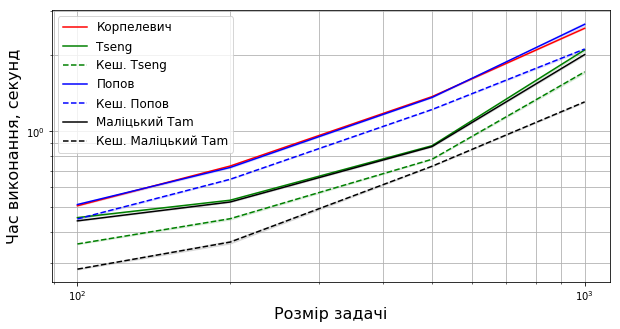
\includegraphics[width=.75\textwidth]{img/2/time.png}
\end{figure}

Та сама інформація у табличці, для зручності:

\begin{table}[H]
	\centering
	\begin{tabular}{|c||c|c|c|c|}\hline
		Розмір задачі & 100 & 200 & 500 & 1000 \\ \hline \hline
		Корпелевич & 0.54 $\pm$ 0.27 & 0.87 $\pm$ 0.30 & 2.39 $\pm$ 0.52 & 7.62 $\pm$ 0.59 \\ \hline
		Tseng & 0.48 $\pm$ 0.27 & 0.77 $\pm$ 0.21 & 1.85 $\pm$ 0.37 & 6.36 $\pm$ 0.77 \\ \hline
		Кеш. Tseng & 0.38 $\pm$ 0.20 & 0.72 $\pm$ 0.11 & 1.40 $\pm$ 0.55 & 4.95 $\pm$ 0.75 \\ \hline
		Попов & 0.49 $\pm$ 0.18 & 1.16 $\pm$ 0.32 & 2.25 $\pm$ 0.69 & 7.79 $\pm$ 1.08 \\ \hline
		Кеш. Попов & 0.34 $\pm$ 0.16 & 0.86 $\pm$ 0.36 & 2.45 $\pm$ 0.40 & 6.39 $\pm$ 0.64 \\ \hline
		Маліцький Tam & 0.49 $\pm$ 0.17 & 0.56 $\pm$ 0.16 & 1.49 $\pm$ 0.48 & 6.10 $\pm$ 0.90 \\ \hline
		Кеш. Маліцький Tam & 0.29 $\pm$ 0.09 & 0.34 $\pm$ 0.06 & 1.19 $\pm$ 0.48 & 3.85 $\pm$ 0.44 \\ \hline
	\end{tabular}
	\caption{Час виконання, секунд}
\end{table}


У цій задачі основна складність все ще у обчисленні оператора $A$, %($O(m^2)$)
хоча обчислення проекції вже більш складне, %($O(m \log m)$)
тому алгоритм Tseng'a має певну перевагу над алгоритмом Попова, який у свою чергу випереджає алгоритм Корпелевич. Щодо кількості ітерацій то усі три алгоритми демонструють практично ідентичні результати.

\begin{table}[H]
	\centering
	\begin{tabular}{|c||c|c|c|c|}\hline
		Розмір задачі & 100 & 200 & 500 & 1000 \\ \hline \hline
		Корпелевич & 1000 $\pm$ 0 & 1000 $\pm$ 0 & 1000 $\pm$ 0 & 1000 $\pm$ 0 \\ \hline
		Tseng & 1000 $\pm$ 0 & 1000 $\pm$ 0 & 1000 $\pm$ 0 & 1000 $\pm$ 0 \\ \hline
		Кеш. Tseng & 1000 $\pm$ 0 & 1000 $\pm$ 0 & 1000 $\pm$ 0 & 1000 $\pm$ 0 \\ \hline
		Попов & 1000 $\pm$ 0 & 1000 $\pm$ 0 & 1000 $\pm$ 0 & 1000 $\pm$ 0 \\ \hline
		Кеш. Попов & 1000 $\pm$ 0 & 1000 $\pm$ 0 & 1000 $\pm$ 0 & 1000 $\pm$ 0 \\ \hline
		Маліцький Tam & 1000 $\pm$ 0 & 1000 $\pm$ 0 & 1000 $\pm$ 0 & 1000 $\pm$ 0 \\ \hline
		Кеш. Маліцький Tam & 1000 $\pm$ 0 & 1000 $\pm$ 0 & 1000 $\pm$ 0 & 1000 $\pm$ 0 \\ \hline
	\end{tabular}
	\caption{Число ітерацій}
\end{table}


Знову ж таки, кешування дає перевагу на великих задачах, хоча вона вже не у 1.5--2 рази. \medskip

\begin{remark}
    Можна кешувати якийсь із матрчиних розкладів $M$ для пришвидшення множення $M x$. 
\end{remark}

\begin{remark}
    Наша реалізація приблизно у 2000 разів швидша за результати наведені у статті \href{https://arxiv.org/abs/1502.04968v1}{[Yura Malitsky, 2015]}. Краща машина, зміна мови програмування та алгоритму проектування на явний є причинами пришвидшення приблизно у співвідношенні $1 : 1 : 2$. 
\end{remark}